\documentclass[11pt]{exam}
% \usepackage{pslatex}
\usepackage{graphicx}
\DeclareGraphicsExtensions{.jpg,.png}
\usepackage{amsmath}
\usepackage{amsfonts}
\usepackage{enumerate}
\firstpageheader{}{}{}
\runningheader{\textbf{Fall 2012}}
 {\textbf{Math 251}}
 {\emph{Page \thepage~of \numpages}}
\runningheadrule
\setlength{\parskip}{1ex}
\setlength{\parindent}{0pt}
\pagestyle{head}
\newcommand{\N}{\mathbb{N}}
\newcommand{\Z}{\mathbb{Z}}
\newcommand{\R}{\mathbb{R}}
\begin{document}

% \printanswers
\addpoints

\noindent
\textbf{{\large Mathematics 251 \\ Exam 1}}
% \hfill Name: \underline{\hspace{0.5in}Answers\hspace{2in}}

\noindent
September 25, 2012  \hfill Name: \underline{\hspace{3in}}


\noindent
\textbf{Instructions}: This exam is closed book: no electronic aids or
printed references are permitted. Justification of all answers is required
for partial credit; please \fbox{\textbf{box}} your final answers. Unless
specifically directed, leave all answers in \textbf{exact form}, e.g.\
$\sqrt{3}$ instead of~$1.732$ and~$\pi/2$ instead of~$1.57$.

Show all pertinent work. \emph{Correct answers without accompanying work will receive little or no credit.} Results from class or from homework or from class can be cited freely. It is in your interest to display your solution in a
clear, readable fashion.

If you need to include more pages, staple them to the back of your exam and make sure that they are clearly labeled by problem number. Indicate in the main body of the exam that your work continues on another page.

Check and make sure you have all of the pages in the
exam; there should be \numpages, including this one. If you have a
question, please raise your hand.

Be sure to read all questions carefully and completely.

\vspace*{2in}

\begin{center}
\gradetable
\end{center}

\vspace*{0.5in}

\begin{center}
{\Large \emph{Good luck!}}
\end{center}

\newpage

\begin{questions}

\question The vector-valued function~$\mathbf{r}(t) = \langle R \cos \omega t, R \sin \omega t \rangle$ parametrizes the circle of radius~$R$ centered at~$(0,0) \in \R^2$ (assume that~$R$,~$\omega > 0$). 

\begin{parts}
\part[8] Consider a particle whose position at time~$t$ is~$\mathbf{r}(t)$ as given above. Verify that the speed of this particle is constant with value~$R \omega$.

%\part[6] Find a formula for the tangent vector~$\mathbf{r}'(t)$ and use it to verify that the speed of a particle whose position is~$\mathbf{r}(t)$ is~$R\omega$.

%\vspace*{2in}

%\part[6] The~\emph{unit} tangent vector~$\mathbf{T}(t)$ is by definition the unique vector of length one that points in the same direction as~$\mathbf{r}'(t)$ (not in the opposite direction). In the notation of the textbook,~$\mathbf{T}(t) = \mathbf{e}_{\mathbf{r}'(t)}$. Find a formula for~$\mathbf{T}(t)$ if~$\mathbf{r}(t)$ is as in the previous part.

%\vspace*{2.5in}

\vspace{\stretch{1}}

\part[10] Use the formula for arc length of a parametrized curve to verify the well-known fact that the circumference of the circle is~$2 \pi R$. (The particle traverses the circle once as~$t$ increases from~$0$ to~$2\pi / \omega$.) \emph{Answers that do not make use of the arc length integral will receive very little credit.}

\vspace{\stretch{1}}

\end{parts}

\newpage

\question Consider a particle moving in the~$(x,y)$-plane whose position at time~$t$ is given for~$0 \leq t \leq 2$ by the parametric equations
\[
c(t) = (3t-1, 4t^2).
\]

\begin{parts}
%\part[8] Find the velocity of the particle at~$t = 2$ (your answer should be a \emph{vector}).
\part[8] Find $dx/dt$ and $dy/dt$, the horizontal and vertical velocities of this particle, at time~$t = 2$ (your answers should be numbers, not vectors).

\vspace{\stretch{1}}

\part[6] Let~$L$ be the line that is tangent to the path of the particle at~$c(2) = (5,16)$. Find the slope of~$L$.

\vspace{\stretch{2}}

\part[12] Find functions~$x(s)$ and~$y(s)$ that parametrize the line~$L$, in other words, such that the point~$(x(s), y(s))$ is on~$L$ for all times~$s$. (The letter~$s$ is used only to distinguish times in this parametrization from times in the parametrization~$c(t)$. The two parametrizations don't have to be related in any way at all.)

\vspace{\stretch{2}}

\end{parts}

\newpage

% \question Consider the \emph{lima\c{c}on} curve pictured below. Its equation in polar coordinates is
% \[
% r = f(\theta) = \frac{1}{2} + \cos{\theta}.
% \]

% \vspace{2in}

% (\emph{Lima\c{c}on} is the French word for ``snail''.)

% \begin{parts}
% \part[12] Use the polar-to-rectangular conversion formulas and~$f(\theta)$ to express~$x$ and~$y$ in terms of~$\theta$ alone (for points on the curve). Find~$dx/d\theta$ and~$dy/d\theta$.

% \vspace*{1.5in}

% \part[6] Your answer to the previous part includes a set of parametric equations for the curve (with parameter the angular coordinate~$\theta$). Write down an equation relating the three derivatives~$dy/dx$, $dx/d\theta$, and~$dy/d\theta$ (hint: chain rule). You don't need to provide any justification here, just the equation suffices.

% \vspace*{1.0in}

% \part[6] There is a unique line tangent to the curve at the origin with positive slope. What is this slope? Use the previous part and a carefully chosen~$\theta$.

% \end{parts}

% \newpage

\question Let~$P = (1,1,0)$, $Q = (0, -1, 1)$, and~$R = (1,-2,2)$. 

% \begin{figure}
% \centering
% \includegraphics[]{}
% \end{figure}

%\vspace*{\stretch{1}}

\begin{parts}
    \part[6] Find the cosine of the angle between the line segments~$\overline{PQ}$ and~$\overline{PR}$.

    \vspace*{\stretch{1}}

    \part[6] Explain why your answer to the previous part means that the points~$P$, $Q$, and~$R$ are the vertices of a triangle (in other words, why the points are not collinear).

    \vspace*{\stretch{1}}

    \part[6] Recall that for \emph{any} two vectors~$\mathbf{u}$, $\mathbf{v}$, the angle formed by~$\mathbf{u}$ and~$\mathbf{v}$ is acute (resp.\ obtuse) if~$\mathbf{u} \cdot \mathbf{v}$ is positive (resp.\ negative). Are any of the angles of the triangle obtuse? Justify your answer.

    \vspace*{\stretch{1}}

    \part[6] Find a vector that is orthogonal to the plane containing the triangle. \emph{Hint.} To contain the triangle, a plane must contain the vectors that connect the triangle's vertices.

    \vspace*{\stretch{2}}
\end{parts}

\newpage

% ~$\ell_1$ be the line in~$\R^3$ containing the points~$(1,1,0)$ and~$(0,-1,1)$. Let~$\ell_2$ be the line containing the points~$(2,1,-2)$ and~$(3,0,-1)$. Find a unit vector that is perpendicular to both~$\ell_1$ and~$\ell_2$.
%\vspace*{4.5in}

\question[8] (Note: In this problem, no justification or explanation is required.) Let~$\mathbf{u}$, $\mathbf{v}$, and~$\mathbf{w}$ be nonzero vectors in~$\R^3$. Identify the correct completion(s) of the sentence: The vectors~$\mathbf{u}$, $\mathbf{v}$, and~$\mathbf{w}$ are coplanar (they lie in one plane) if (select one of (a) through (g)):
\begin{figure}[ht]
\hspace{2cm}
\begin{minipage}[t]{0.55\linewidth}
\begin{enumerate}[I.]
    \item One of the three vectors is parallel to the cross product of the others.
    \item There exist scalars $a$ and $b$ with $\mathbf{w} = a \mathbf{u} + b \mathbf{v}$.
    \item $(\mathbf{u} \times \mathbf{v}) \times \mathbf{w} = \mathbf{0}$.
    \item $\mathbf{u} \cdot (\mathbf{v} \times \mathbf{w}) = 0$.
\end{enumerate}
\end{minipage}
\hspace{0.5cm}
\begin{minipage}[t]{0.35\linewidth}
\begin{enumerate}[a.]
    \item I only
    \item II only
    \item III only
    \item II and IV only
    \item III and IV only
    \item II, III, and IV only
    \item I, II, III, and IV
\end{enumerate}
\end{minipage}
\end{figure}
\question[12] Suppose that $\mathbf{u}$ and $\mathbf{v}$ are orthogonal. Use facts about vectors and their dot products to verify the equation
\[
     ||\mathbf{u} + \mathbf{v}||^2 = ||\mathbf{u}||^2 + ||\mathbf{v}||^2.
 \] 
Do you think this equation can be true for a pair of non-orthogonal vectors? Justify your answer.

\vspace*{\stretch{1}}

\newpage

\question[12] Calculate the magnitude of the force (in $\mathrm{N} = \mathrm{kg}\cdot\mathrm{m}/\mathrm{s}^2$) required for Val to push a $10$ kg squirrel up a frictionless incline as pictured. Assume Val exerts force parallel to the direction of travel up the ramp, and try not to think about what might happen to her. Assume that the acceleration $g$ due to gravity is 9.8 $\mathrm{m}/\mathrm{s}^2$. You do not have to simplify your answer.

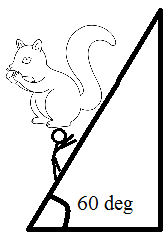
\includegraphics[width=82px,height=117px]{f12_exam1_fig1}

\vspace*{\stretch{1}}

\end{questions}

\end{document} 